\documentclass[]{beamer}
%\documentclass[9pt]{beamer}


\mode<presentation>
{
\usetheme{Singapore} %use default if problems or  Singapore or
  % or ... https://deic-web.uab.cat/~iblanes/beamer_gallery/index_by_theme.html
\usefonttheme{serif}
}
\setbeamertemplate{footline}[frame number]
\usepackage{booktabs}
\usepackage{color}

\usepackage[english]{babel}
% or whatever

\usepackage[latin1]{inputenc}
% or whatever

\usepackage{times}
\usepackage[T1]{fontenc}
% Or whatever. Note that the encoding and the font should match. If T1
% does not look nice, try deleting the line with the fontenc.
\usepackage[super]{nth}
\usepackage{xcolor}
\usepackage{relsize} %large math

\usepackage{graphicx} % to insert the logo

\usepackage{hyperref}
\hypersetup{
  colorlinks   = true, %Colours links instead of ugly boxes
  urlcolor     = blue, %Colour for external hyperlinks
  linkcolor    = blue, %Colour of internal links
  citecolor   = red %Colour of citations
}

\usepackage[font=scriptsize,skip=1pt]{caption}

\setbeamertemplate{caption}[numbered]

\title{Uno schema e alcuni link utili}

\author[] % (optional, use only with lots of authors)
{Pietro colpevole \ldots non unico}
% - Give the names in the same order as the appear in the paper.
% - Use the \inst{?} command only if the authors have different
%   affiliation.


\date[] % (optional, should be abbreviation of conference name)
{Rivoli -- 12 febbraio 2022}

\begin{document}

%%%%%%%%%%%%%%%%%%%%%%%%%%%%%%%%%%%%%%%%%%%%%%%%%%%%%%%%%
\begin{frame}


\titlepage


\end{frame}

%%%%%%%%%%%%%%%%%%%%%%%%%%%%%%%%%%%%%%%%%%%%%%%%%%%%%%%%%
\section{Uno schema ABMi}

%%%%%%%%%%%%%%%%%%%%%%%%%%%%%%%%%%%%%%%%%%%%%%%%%%%%%%%%%
\begin{frame}{~} % 1



\begin{figure}[H]
\center
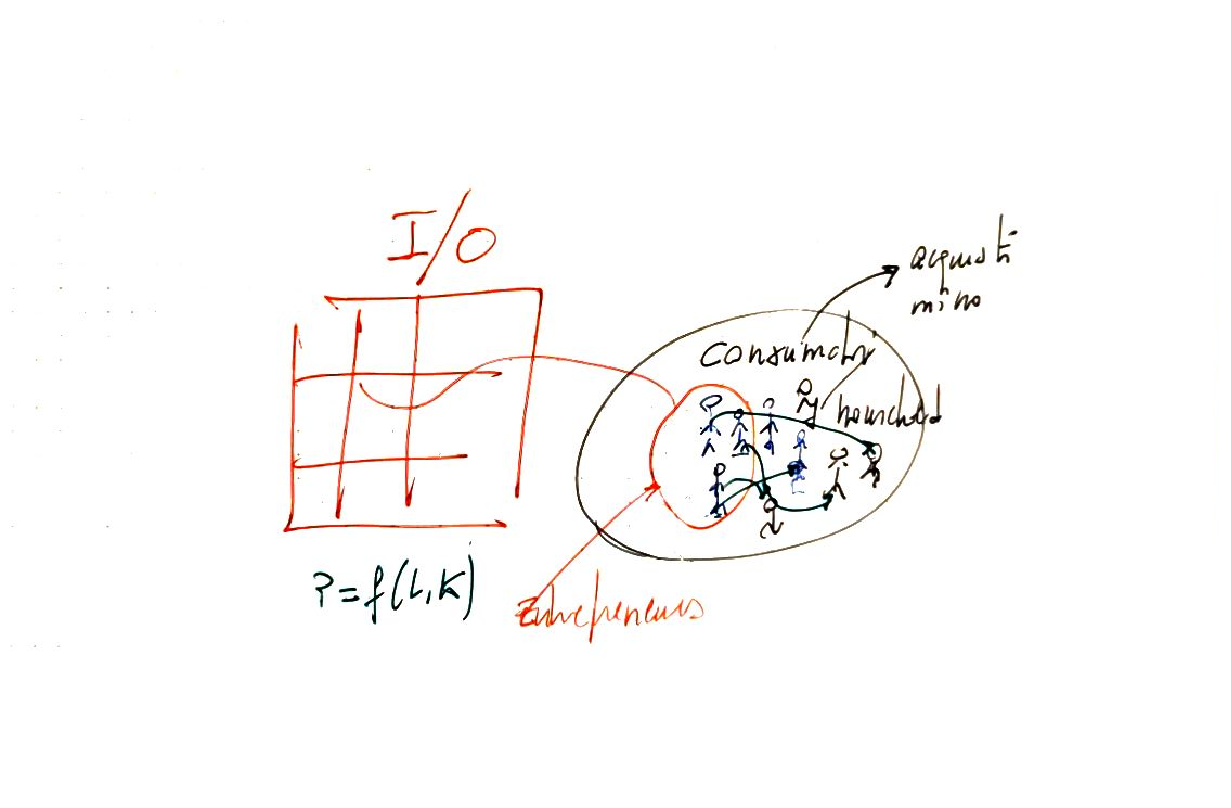
\includegraphics[scale=0.50]{1.pdf}
\label{1}
\caption{Produzione e consumo micro micro}
\end{figure}

\end{frame}

%%%%%%%%%%%%%%%%%%%%%%%%%%%%%%%%%%%%%%%%%%%%%%%%%%%%%%%%%
\begin{frame}{~} % 2



\begin{figure}[H]
\center
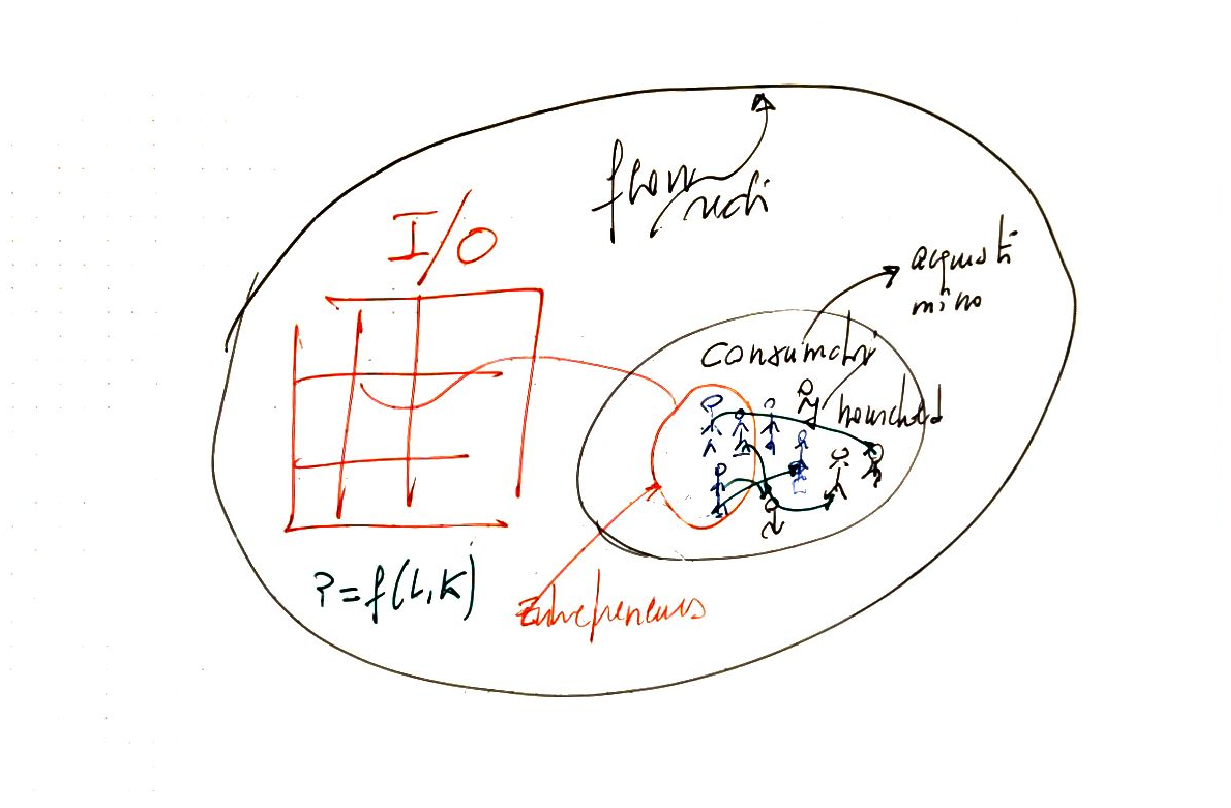
\includegraphics[scale=0.50]{2.pdf}
\label{2}
\caption{Quadratura flussi reali, con produzione, consumi e \ldots}
\end{figure}

\end{frame}

%%%%%%%%%%%%%%%%%%%%%%%%%%%%%%%%%%%%%%%%%%%%%%%%%%%%%%%%%
\begin{frame}{~} % 3



\begin{figure}[H]
\center
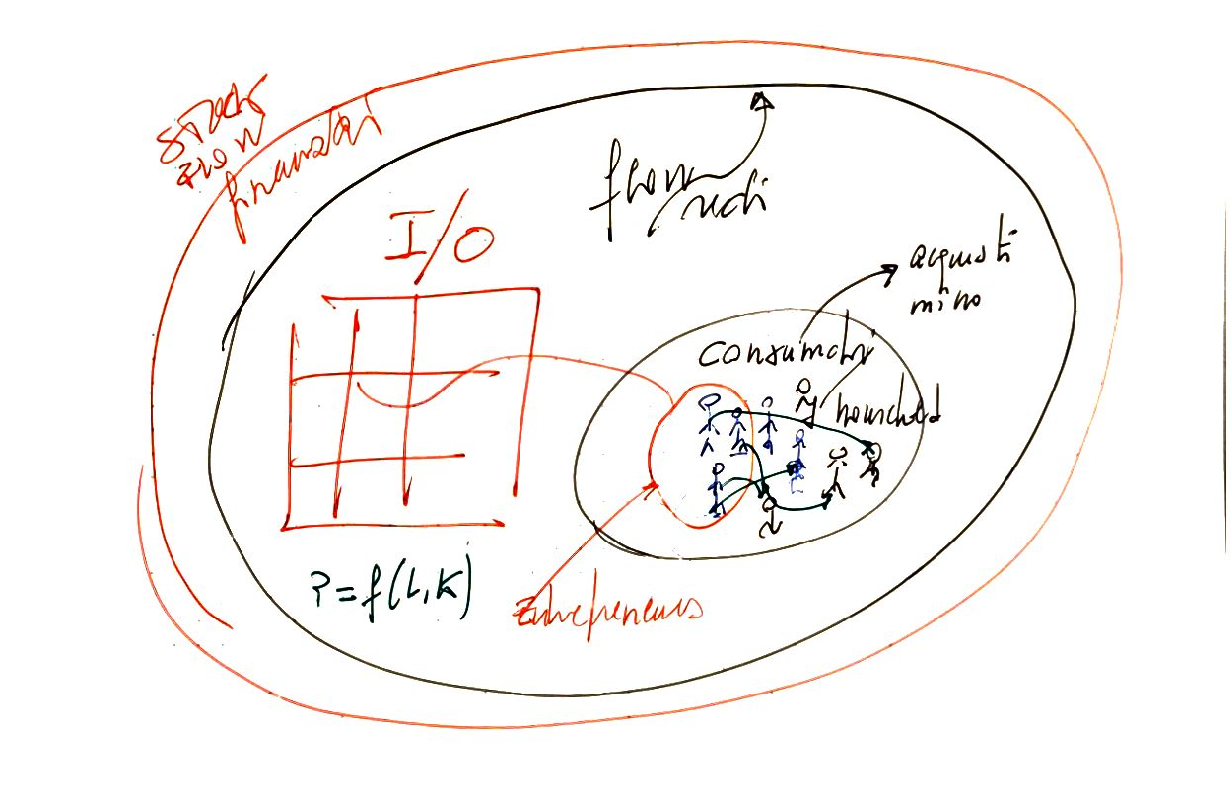
\includegraphics[scale=0.50]{3.pdf}
\label{3}
\caption{Quadratura stock flussi finanziari, con produzione, consumi e \ldots}
\end{figure}

\end{frame}

%%%%%%%%%%%%%%%%%%%%%%%%%%%%%%%%%%%%%%%%%%%%%%%%%%%%%%%%%
\begin{frame}{~} % 4



\begin{figure}[H]
\center
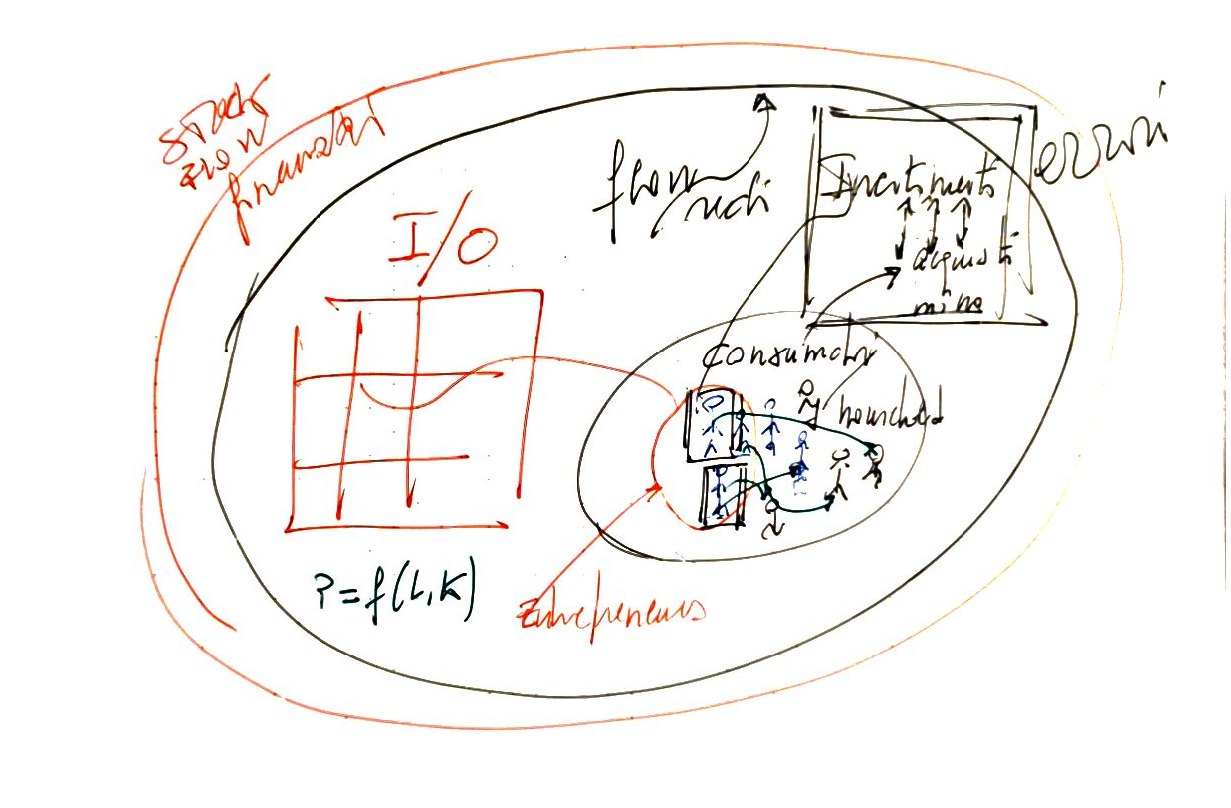
\includegraphics[scale=0.50]{4.pdf}
\label{4}
\caption{\ldots investimenti}
\end{figure}

\end{frame}

%%%%%%%%%%%%%%%%%%%%%%%%%%%%%%%%%%%%%%%%%%%%%%%%%%%%%%%%%
\begin{frame}{~}



\begin{figure}[H]
\center
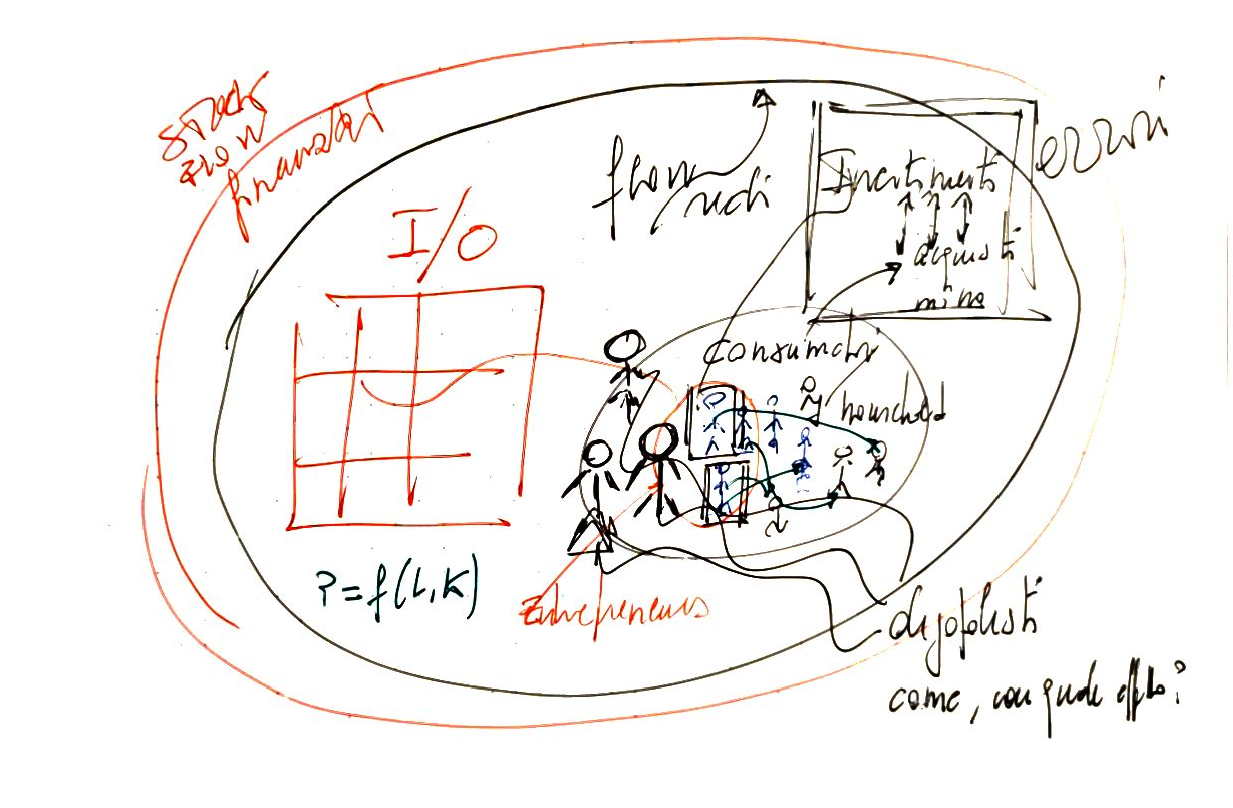
\includegraphics[scale=0.50]{5.pdf}
\label{5}
\caption{Con oligopolisti}
\end{figure}

\end{frame}

%%%%%%%%%%%%%%%%%%%%%%%%%%%%%%%%%%%%%%%%%%%%%%%%%%%%%%%%%
\begin{frame}{~} % 6



\begin{figure}[H]
\center
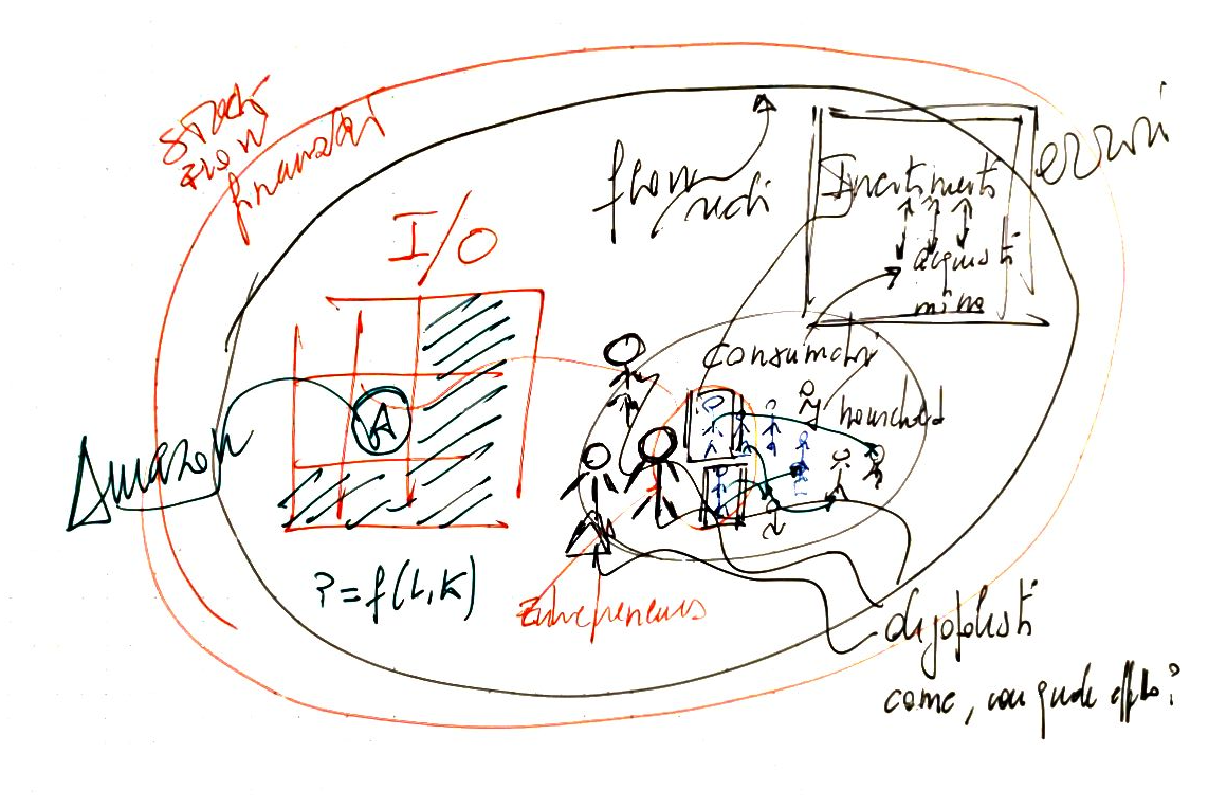
\includegraphics[scale=0.50]{6.pdf}
\caption{Sovrapposizione produzione industriale e commercializzazione e \ldots CHI DECIDE CHE COSA PRODURRE?}
\label{6}
\end{figure}

\end{frame}


%%%%%%%%%%%%%%%%%%%%%%%%%%%%%%%%%%%%%%%%%%%%%%%%%%%%%%%%%
\begin{frame}{~} % 7



\begin{figure}[H]
\center
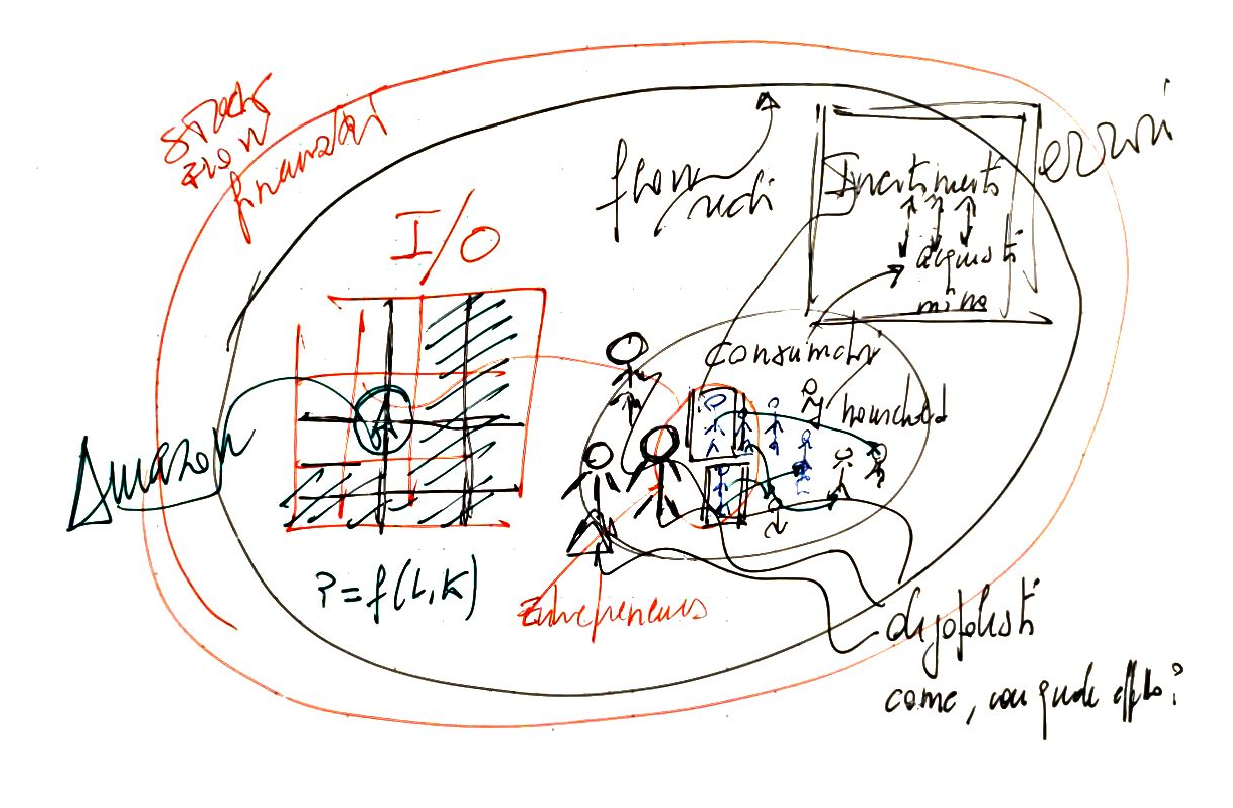
\includegraphics[scale=0.50]{7.pdf}
\label{7}
\caption{Produzione e commercializzazione distinte per beni durevoli e beni investimento}
\end{figure}

\end{frame}

%%%%%%%%%%%%%%%%%%%%%%%%%%%%%%%%%%%%%%%%%%%%%%%%%%%%%%%%%
\section{Linksi}

%%%%%%%%%%%%%%%%%%%%%%%%%%%%%%%%%%%%%%%%%%%%%%%%%%%%%%%%%
\begin{frame}{Queste slide, Overleaf e GitHub}

Links

\end{frame}

\end{document}
